\documentclass[11pt,letterpaper,twocolumn]{article}

\usepackage{xcolor,graphicx,multicol,tabularx,array,pdfpages,tikz,pgfplots,colortbl}
\usepackage[top=1.0in, bottom=1.0in, left=1.0in, right=1.0in]{geometry}
\usepackage[margin=10pt, font=small, labelfont=bf]{caption}
\usepackage[binary-units]{siunitx}

\renewcommand{\familydefault}{\sfdefault}
\renewcommand\textbullet{\ensuremath{\bullet}}
\renewcommand\thefootnote{\arabic{footnote}}
\pgfplotsset{compat=1.12}

\newcolumntype{C}{>{\centering\arraybackslash}p{4em}}

\begin{document}

\twocolumn[{
\begingroup
    \centering
    \huge \textbf{Paradigms and Applications of the Arduino Uno} \\ [.25em]
    \large \textbf{Computer Engineering 3150 Research Paper} \\ [.5em]
    \Large Illya Starikov  \\ [.5em]
\endgroup
}]

\section{Introduction}
The Arduino is an open-sourced family of microcontrollers aimed at not just the specialist, but also the hobbyist or enthusiast. With a multi-platform\footnote{Supported on MAC OS X, Linux, and Windows.} IDE (Integrated Development Environment) provided and maintained by Arduino, code can be written and deployed within seconds, making it easy for anyone to get started. A ``hello world''-esque program (cause an led light to flash on and off) can be implemented in only 12 lines of code\footnote{Excluding \texttt{int main()} and preprocessor directives.} \cite{book}.

\begin{verbatim}
int ledPin = 10;

void setup() {
    pinMode(ledPin, OUTPUT);
}

void loop() {
    digitalWrite(ledPin, HIGH);
    delay(1000);
    digitalWrite(ledPin, LOW);
    delay(1000);
}
\end{verbatim}

\noindent Anyone familiar with C or C++ can get started by briefly skimming documentation. However, the flexibility of and power of Arduino's microcontrollers is why professionals use it.

What makes Arduino so powerful is its ease of expandability, a process known as shielding. Such shields can be provide additional functionality, such as: \cite{shields}

\begin{itemize}
    \item Bluetooth
    \item Internet connectivity via WiFi or Ethernet
    \item Sound and speech synthesizer
    \item Allowing a stack of Arduino boards to communicate
\end{itemize}

\noindent This readily available power of any other board makes Arduino ideal for any project. And if the functionality is not there, producing one is fairly simple --- design a PCB (print circuit board) and mount it.

As mentioned prior, Arduino open sources everything; by everything, this covers to code, schematics, and designs. Because of the open source license (Creative Commons Attribution Share-Alike), it is possible to entirely replicate the board\footnote{Excluding the name Arduino or Uno}. This is actually a common occurrence, giving rise to Arduino ``clones'', such as the Aliexpress and Teensy --- of course, the Arduino Uno (the topic of this paper) is also a ``clone''\footnote{Based on the technology of the ATmega328.} of ATmega328.

\subsection{The Arduino Uno}
The Arduino Uno is an 8-bit microcontroller with \SI{32}{\kilo\byte} of flash storage and \SI{2}{\kilo\byte} of RAM (Random Access Memory). Because it operates at \SI{5}{\volt}, it can be charged through the provided power jack or a typical \SI{5}{\volt} charging block (e.g. a typical phone charger), or a \SI{7}{\volt} - \SI{12}{\volt} input pin.\footnote{However, the pin ``bypasses the regulator, and can damage your board.'' It is not advised charging anywhere out of the recommended range}. As for as analog controls and peripherals, the Uno has ``14 digital input/output pins (of which 6 can be used as PWM outputs), 6 analog inputs, a 16 MHz ceramic resonator, a USB connection, a power jack, an ICSP header, and a reset button'' \cite{specs}. Another great feature is the price: \$\num{29.95}.

\begin{figure}[!h]
    \centering
    \includegraphics[width=.90\columnwidth]{arduino-uno.jpg}
    \caption{The Arduino Uno Microcontroller \cite{image}.}
\end{figure}

Because of its open-sourcing and given the \num{6} years to mature \cite{blogpost}, the Uno has gather quite a community on the internet. The forums, hosted on the Arduino website, are active with some threads reaching up to \num{100000} posts. Topics include \cite{forums}:

\begin{itemize}
    \item Robotics (``Platforms, motors, algorithms and sensors to conform robotics projects'')
    \item Home Automation and Networked Objects (Internet of Things)
    \item E-Textile and Craft (``flexible conductive materials, electroluminiscent materials'')
    \item Device Hacking (``reappropiation of devices, tricks of the trade'')
\end{itemize}

\section{Applications of The Arduino Uno}
The Arduino Uno's flexibilty makes it pragmatic to be used in a wide array of industries; three of these industries are Education, Healthcare, and Home Automation.

\subsection{Education}
In the education market, there are many factors that are needed to accounted for in adopting new technology, and the Arduino Uno usually accommodates for these factors, typically making it an ideal candidate. The two most important factors are affordability and ease of use.

When considering purchasing equipment, price is the most important element. Students need to have the ability to experiment with technology without fear of breaking it; not only that, but there is maintenance, replacement and installation costs associate with it. Fortunately, the Uno fits this niche. As aforementioned, the Uno is competitively at \$\num{29.95}. The Arduino Starter Kit, which not only contains the Uno, but many sample projects that gives a hand-on experience with it, costs \$\num{99.99} Lastly, the multiple shields that can be purchased range form \$\num{1.00} to little over \$\num{100}, but most usually lower than \$\num{40}.

For such a competitive price, the Uno still manages to have a lot of thought and consideration with regards to the user. The cross-platform IDE ensures frictionless setup; programming the microcontroller can begin immediately after installation. The online documentation and forums are house enough information to get started with any kind of project. This makes the Arduino Uno the ideal microcontroller to get started with.

This was the mentality behind a team of researches from Federal University of Rio Grande do Sul Porto Alegre-Rs and Criciúma-Sc  from Brazil. In a recent attempt to further engage electrical engineering students, the group built a ``remote educational experiment of a current motor (DC motor) control speed, which allow the students to interact with the control systems P, PI, PID applied to the rotation control of the remote mode engine'' \cite{engineering}.

Instead of being constrained to the labs, where traditional equipment is kept, the researches moved the lab online where it is accessible from anywhere at anytime. The user can, through an online Java application, access the hardware in the lab. The user interaction is still natural, because the application is tethered to a camera that sends a continuous live video that will be streamed to the user's browser. The user can send live commands to the device, and get instantaneous feedback. As the user is interacting with the application, the commands are being sent to the Arduino microcontroller, which is not only controlling the engine, but is acting as a PID control machine.

\begin{figure}[!ht]
    \centering
    \includegraphics[width=.90\columnwidth]{pid-controller.pdf}
    \caption{The Java applet, with the livestream on the left and PID controls on the right \cite{engineering}.}
\end{figure}

A PID controller (proportional-integral-derivative) is a self-correcting feedback mechanism that asymptotically approaches a stable point, also referred to as a setpoint. The error correcting equation, as a function of time, is a integro-differential equation as such:

\begin{equation}
    u(t) = k_p e(t) + K_i \int _0 ^t e(\tau) \ d\tau + K_d \frac{d \ e(t)}{dt}.
\end{equation}

It reads ``as the error tolerance at a set time $u(t)$ is calculated by the current error ($k_p e(t)$) with the potential error that needs to be considered ($K_i \int e(\tau) \ d\tau$), while taking away the excess error ($K_d \frac{d \ e(t)}{dt}$)''. As this function changes with respect to time, the system (in this case, the DC motor) calculates the error and asymptotically reaches a setpoint. In this case, the PID controller tries to regulate the voltage and bring the engine to a steady state. And the Uno does all of the calculations in real time and lets the user see at a glance what the each state (P, I, or D) is at, and what the setpoint is.

And at the end of the session, a majority of the participants enjoyed the project. The original goal of further engaging students outside of the classroom was achieved; the project was an overwhelming success.

\begin{table}[!h]
  \begin{tabularx}{\linewidth}{|C|C|C|C|}
    \hline \rowcolor{lightgray}
    \multicolumn{4}{|X|}{Experiment contributed to better understanding the concepts developed in the discipline of control systems?} \\
    \hline

    Excellent & Good & Regular & Bad \\
    43\% & 36\% & 11\% & 10\% \\

    \hline \rowcolor{lightgray}
    \multicolumn{4}{|X|}{What is your impression about developing experiments remote related to control systems?} \\
    \hline

    Excellent & Good & Regular & Bad \\
    40\% & 38\% & 14\% & 8\% \\

    \hline \rowcolor{lightgray}
    \multicolumn{4}{|X|}{In your opinion greater learning control systems in the development of activities linked to experiments remote or simulations?} \\
    \hline

    \footnotesize Simulation & \footnotesize Real experiments & \footnotesize Both & \footnotesize Combination \\
    5\% & 27\% & 44\% & 24\% \\ \hline

  \end{tabularx}

  \caption{Satisfaction of the PID controller project \cite{engineering}.}
\end{table}

However, this is only one of the many interesting projects --- all of which don't have to be a strict application to Electrical Engineering. A group of researches from IBM decided to target a younger age-group: \num{9}\textsuperscript{th}--\num{12}\textsuperscript{th} grade students. Seeing as this was the age group that had a rapid loss of interest in STEM (Science, Technology, Engineering, and Mathematics) based fields, the IBM group realized this was a delicate experiment. The experiments could not be too technical, because of the lack of knowledge and experience in high schools, but could not be mundane; all of this had to be considered while trying to teach students the basics of electronics and programming.

The students received hands-on experience by doing a simplified experiment: programming a blinking LED light; and then further expanding this concept by placing the LED lights to a bag and making text light up. The researches said the students ``were very engaged to and excited about open source, which is affordable and accessible. The students conducted the experiments with no major issues, except the lack of time'' \cite{students}.

After the experiment, there were presentations of the more advanced things that could be done. Some of these were: a Twitter client that projects negative or positive feelings in regards to an debated topic, a toy car that could be controlled with a PlayStation controller, and even a quadcopter. All of these demonstrations were powered with the Arduino Uno and a couple of shields.

The IBM group is continuing to expand this project in the coming years and hoping to educate more high school students about the power of programming, electronics, and open source.

\subsection{Healthcare}
As previously mentioned, the Arduino Uno is based on the ATmega328P, the high performance microcontroller from Atmel. However, performance is not exclusively what the team at Arduino focused on; they weighed performance with reliability. This blend of high performance and reliability makes the Arduino Uno a suitable microcontroller to be used in healthcare. Two graduate students at the Institute of Biophysics and Biomedical Engineering in Portugal have found an interesting use for it: hand rehabilitation therapy.

Because modern, technological approaches to hand rehabilitation therapy have been proven to be quite expensive and needed heavy technical experience and support, the team decided to make an affordable and simple system that can used at the comfort of your own home. It's called a ``hand therapist''.

The team started with Unity3D, a popular game engine, to simulate an environment on a personal computer. The environment is essentially a canvas with a working hand that be controlled with a series of commands in the $xyz$-plane, making it easy to wire up a working hand to a microcontroller to interpret said commands; and that's exactly what the team did.

The Uno interprets the movement and synchronously plots the movement on the computer. Then the user can ``grab, hold, transport and drop a cube in several increasingly difficult puzzle levels''. Not only does this make hand therapy much easier, but more affordable (less than \$\num{600}) \cite{hand}.

\begin{figure}[!ht]
    \centering
    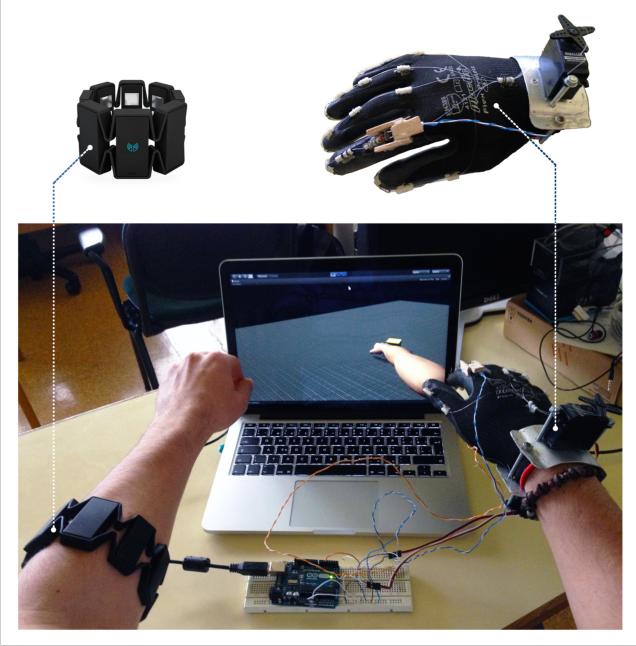
\includegraphics[width=.90\columnwidth]{hand-therapist.pdf}
    \caption{The rehabilitation system \cite{hand}.}
\end{figure}

But complicated hand therapy is not the only application for the Uno in healthcare. Another research team in India have managed to hook up a microcontroller to monitor patient heartrate through the course of the day with an Uno and a bright LED light and transmit the information to the doctor at a fixed schedule, making it easy to regularly check up on patients \cite{heartrate}.

Thanks to the Uno, not only is healthcare becoming more reliable, but less expensive too.

\subsection{Home Automation}
Today's technology is significantly more advanced then ever; devices are getting smarter, better at communicating, and even more efficient. Something that came out of this ``technological revolution'' is the idea of a smarthome --- powered by the IoT (Internet of Things). A smarthome is nothing more than a home ``that constitutes advanced automation systems to provide the occupants with sophisticated monitoring and controlling over the different functions of the building'' \cite{iot}.

Home automation is a very broad topic, ranging from things such as temperature monitoring to motion tracking to light automation; fortunately, the Arduino Uno can do all of the above. Researchers from MIT managed to mount input/output blocks consisting of ``PIR (Passive Infra-Red) motion sensor, LDR (Light Dependent Resistor) and an LM35 temperature sensor as inputs and some lamps'' and get the blocks communicating.

The PIR motion sense was to detect motion; not only could it turn lights on/off (via the LDR) if anyone was present, but it could act as a security system as well. If there was any suspicious movement during irregular hours, an alarm is buzzed. This buzzing acts as a warning system to any intruders or potential wild animals. The LM35 is not only to monitor temperature, but to enable and Air Conditioning or fans when a certain temperature threshold has been reached.

\begin{figure}
    \centering
    \begin{tikzpicture}
        \begin{axis}[
            scale only axis,
            width=.8\columnwidth,
            height = 5cm,
            title={Temperature Measurement},
            xlabel={Time (Seconds)},
            ylabel={Temperatures ($^{\circ}$C)},
            legend pos=north west,
            ymajorgrids=true,
            grid style=dashed,
            ymin = 23,
            ymax = 24.5
        ]

        \addplot[color=blue, mark = square ] table [x=a, y=b, col sep=comma] {temperatures.csv};
        \addlegendentry{Temperature}
    \end{axis}
    \end{tikzpicture}

    \caption{The system usually keeps the room within a $1^{\circ}\text{C}$.}
\end{figure}

What makes these sensor different than switches on the wall or a regular AC controller is these can be monitored, synchronously, virtually. The current front-end is a MATLAB GUI (Graphical User Interface). Instead of having to traverse the typical household, the entire system is a few clicks away. This makes the entire household not only systematic and tidy, but more cost and energy efficient; and because it runs on a \SI{5}{volt} Arduino Uno, it is using significantly less power than the AC unit, lighting, and security systems\footnote{However, the energy efficiency should be traded for one's safety.}.

\section{Conclusion}
As laid out previously, the Arduino Uno has incredible uses in three major fields: Education, Healthcare, and Home Automation. The Uno's ease of use makes it an ideal electronic to get interest in Engineering-based fields, while it's price makes a candidate to be used in the classroom without fear of breaking hardware. The reliabilty and processing power makes it a great aid in healthcare, such as ``hand therapy'' or monitoring a patient status. Also, the Uno is great at home automation, where it can simultaneously monitor movement, temperature, and lighting based on room occupancy. Looking forward, one can surely expect many more great microcontrollers from Arduino that will get be in many, interesting ways.

\begin{thebibliography}{1}
    \bibitem{book} M. McRoberts, {\it Beginning Arduino}.

    \bibitem{shields} ``Arduino - ArduinoShields'', {\it Arduino.cc}, 2016. [Online]. Available: https://www.arduino.cc/en/Main/arduinoShields. [Accessed: 11- Sep- 2016].

    \bibitem{specs} ``Arduino - ArduinoBoardUno'', {\it Arduino.cc}, 2016. [Online]. Available: https://www.arduino.cc/en/Main/ArduinoBoardUno. [Accessed: 11- Sep- 2016].

    \bibitem{image} ``Arduino Uno'', {\it Wikimedia}, 2016. [Online]. Available: https://upload.wikimedia.org/wikipedia/ commons/9/90/Barbone\_Arduino\_Uno.jpg. [Accessed: 11- Sep- 2016].

    \bibitem{blogpost} M. Banzi, ``Arduino Blog – Dinner is Ready'', {\it Blog.arduino.cc}, 2010. [Online]. Available: https://blog.arduino.cc/2010/09/24/dinner-is-ready/. [Accessed: 11- Sep- 2016].

    \bibitem{forums} ``Arduino Forum - Index'', {\it Forum.arduino.cc}, 2016. [Online]. Available: http://forum.arduino.cc. [Accessed: 11- Sep- 2016].

    \bibitem{engineering} J. M. Neto, S. Paladini, C. E. Pereira and R. Marcelino, ``Remote educational experiment applied to electrical engineering,'' {\it Remote Engineering and Virtual Instrumentation (REV)}, 2012 9th International Conference on, Bilbao, 2012, pp. 1-5.

    \bibitem{students} L. M. Herger and M. Bodarky, ``Engaging students with open source technologies and Arduino,'' {\it Integrated STEM Education Conference (ISEC)}, 2015 IEEE, Princeton, NJ, 2015, pp. 27-32.

    \bibitem{hand} R. Lipovský and H. A. Ferreira, ``Hand therapist: A rehabilitation approach based on wearable technology and video gaming,'' {\it Bioengineering (ENBENG)}, 2015 IEEE 4th Portuguese Meeting on, Porto, 2015, pp. 1-2.

    \bibitem{heartrate} P. A. Pawar, ``Heart rate monitoring system using IR base sensor \& Arduino Uno,'' {\it IT in Business, Industry and Government (CSIBIG)}, 2014 Conference on, Indore, 2014, pp. 1-3.

    \bibitem{iot} A. R. Behera, J. Devi and D. S. Mishra, ``A comparative study and implementation of real time home automation system,'' {\it 2015 International Conference on Energy Systems and Applications}, Pune, 2015, pp. 28-33.
\end{thebibliography}


\end{document}